\documentclass{article}

\usepackage{bm}
\usepackage{harpoon}
\usepackage{listings}
\usepackage[left=2cm, right=2cm]{geometry}
\usepackage{setspace}
\usepackage{bm}
\usepackage{cmap}
\usepackage{cite}
\usepackage{float}
\usepackage{stmaryrd}
\usepackage{amsthm}
\usepackage{amsmath}
\usepackage{amssymb}
\usepackage{setspace}
\usepackage{enumerate}
\usepackage{indentfirst}
\usepackage{fontspec}
\usepackage{booktabs}
\usepackage{tikz}
\usepackage{subfigure}
\usepackage{graphicx}
\usetikzlibrary{arrows,decorations}
\usepackage[colorlinks, linkcolor=red]{hyperref}
\usepackage[indentfirst]{xeCJK}
\setCJKmainfont[BoldFont={SimHei},ItalicFont={KaiTi}]{SimSun}
\setCJKsansfont{KaiTi}

\setCJKfamilyfont{KaiTi}{楷体}
\newcommand{\kai}{\CJKfamily{KaiTi}}

\allowdisplaybreaks
\newfontfamily\Courier{Courier New}
\renewcommand{\figurename}{图}

\def\ack{\section*{Acknowledgements}%
  \addtocontents{toc}{\protect\vspace{6pt}}%
  \addcontentsline{toc}{section}{Acknowledgements}%
}

\lstset{
	language=C++,
	tabsize=4,
	numbers=left,
	breaklines=tr,
	extendedchars=false
	xleftmargin=0em,
	xrightmargin=0em,
	aboveskip=1em,
	numberstyle=\small\Courier,
    basicstyle=\small\Courier
}

\renewenvironment{abstract}{
\subsection*{\textbf{摘~~要}}
\kai
}{}

\renewcommand{\contentsname}{\large 目~~录}

\newenvironment{keywords}{
\large\noindent\textbf{关键词}\,\,
}{\kai}
\begin{document}
	\title{\textbf{基于OpenGL$^{\text{TM}}$的物理引擎实现及应用}}
	\author{黎金宁\,\,秋闻达\,\,谭博文\\胥拿云\,\,许臻佳\,\,杨嘉成}
	\maketitle
	\begin{abstract}
		OpenGL$^{\text{TM}}$是行业领域中最为广泛接纳的2D/3D图形API\cite{ref2},其自诞生至今已催生了各种计算机平台及设备上的数千优秀应用程序。OpenGL$^{\text{TM}}$是独
		立于视窗操作系统或其它操作系统的,亦是网络透明的。在包含CAD、内容创作、能源、娱乐、游戏开发、制造业、制药业及虚拟现实等行业领域中,OpenGL$^{\text{TM}}$帮助程序员
		实现在PC、工作站、超级计算机等硬件设备上的高性能、极具冲击力的高视觉表现力图形处理软件的开发。本文作者编写了一种建立在OpenGL$^{\text{TM}}$上的物理引擎
		\cite{ref1},并且用该物理引擎探究了热力学和三体问题等物理问题,本文将从该物理引擎的实现出发,描述整个引擎的算法,并且将给出模拟实验结果。
	\end{abstract}
	\tableofcontents
	\newpage
	\section{OpenGL$^{\text{TM}}$概述}
	\subsection{工作机制}
	\indent 假设现在我们有一副物理图像需要显示在电脑屏幕上,那么首先我们会将这份物理图像的细节传输到OpenGL$^{\text{TM}}$的缓冲区中,之后OpenGL$^{\text{TM}}$根据缓冲区
	中数据,进行渲染工作(即将缓冲区中的数据转化为图像),最后通过交换缓存区(glutSwapBuffers)操作将图像显示在屏幕上。\par
	值得注意的是,这个工作机制决定了之后的引擎的工作机制,即引擎应该给出每个时刻的物理图像,而非只给出关键的事件点,OpenGL$^{\text{TM}}$只能从一个时刻过渡到和它紧邻的下
	一个时刻,而不能跳跃地从一个事件过渡到另外一个事件。
	具体步骤如下图所示:
	\begin{figure}[!htbp]
		\centering
		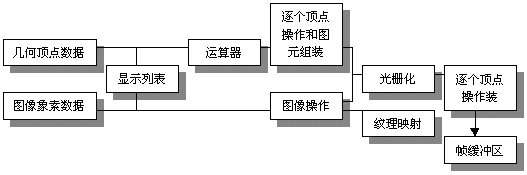
\includegraphics[width=15.5cm]{graph1.jpg}
	\end{figure}
	\subsection{评价}
	根据之后的实验结果,我们发现OpenGL$^{\text{TM}}$具有如下几个特点(优点/缺点):
	\begin{itemize}
		\item 相比其他的Graphics API(例如Microsoft DirectX),OpenGL$^{\text{TM}}$兼容性极强,同一份代码基本能够同时在Windows和Linux操作系统上编译并且达到基本相同的效果;
		\item OpenGL与C++能够紧密结合,将C++的运算速度这个优点和OpenGL$^{\text{TM}}$强大的渲染机制结合起来,增强了计算速度。和WebGL$^{\text{TM}}$与JavaScript的组合相
		比,OpenGL$^{\text{TM}}$和C++的组合显然更具有竞争力;
		\item OpenGL$^{\text{TM}}$操作图像相对麻烦,同时在绘制轨迹的时候只能保存下轨迹之后再逐步绘制,一定程度上影响的绘制图像的效率;
		\item OpenGL$^{\text{TM}}$是过程性的API,因而OpenGL$^{\text{TM}}$不支持面向对象编程,一定程度上影响了编写程序时的分工与代码可读性;
		\item C++不能很好地将图表纳入程序中,因此实验的具体结果只能在模拟计算之后再进行分析。
	\end{itemize}
	\newpage
	\section{驱动引擎}
	\subsection{分子动力学引擎}
	\subsubsection{分子动力学方法}
	\indent 分子动力学法(MD方法,Molecular Dynamics Method),是用计算机模拟的一种,是调查物质诸性质时候使用的手法之一。根据在计算机中每时每刻的追踪全部的粒子的运动的规
	律,导出物质全体的性质这就是分子动力学法。\par
	\indent 分子动力学法是要严格求解每个粒子的运动方程,通过分析系统来确定粒子的运动状态。MD方法一般认为粒子服从牛顿运动规律,粒子所受到的作用力通过粒子间相互作用势计算,
	因此粒子的初始条件和运动方程中的受力状况一旦确定,系统就可被精确求解。
	\subsubsection{评价}
	\begin{itemize}
		\item 编程复杂度较低,基本上只需要给出运动方程就能够模拟;
		\item 灵活性高,在之后将会看到分子动力学方法作为了大部分引擎的内核;
		\item 计算速度较慢,因为每次显示都需要重新计算每个分子的受力情况;
		\item 模拟精度较差,如果采用的硬球势,那么就很有可能会出现两个分子对穿而过的情况;
	\end{itemize}
	\subsection{事件驱动引擎}
	如果不考虑$n$个原子的其他相互作用(即只有碰撞),那么考虑我们现在有一个指针表示当前显示的图像所对应的时刻,如果当前时刻小于下一个碰撞,那么所有原子都向它所在的那个
	方向运动一个极小的时间$\mathrm{d}t$,否则我们按照动量守恒改变每个例子的速度
	\subsubsection{碰撞判定}
	\subsubsection*{球与球的碰撞}
	假设有两个小球,中心位置分别是$\mathbf{r_1}(x_1,y_1)$,$\mathbf{r_2}(x_2,y_2)$,速度分别是$\mathbf{v_1}(v_{x_1},v_{y_1})$,$\mathbf{v_2}(v_{x_2},v_{y_2})$,半径
	分别是$r_1$,$r_2$。以球1为参考系,将球1中心位置作为新的坐标系的原点,则球2的中心坐标变为$\mathbf{r_2'}(x_2-x_1,y_2-y_1)$,速度变
	为$\mathbf{v_2'}(v_{x_2}-v_{x_1},v_{y_2}-v_{x_1})$。考虑到相撞即为球心距为$d_1+d_2$,所以可以将球2看作点,球1的半径变
	为$d_1'=d_1+d_2$。得到方程:
	\[|\mathbf{r_2'}+t\mathbf{v_2'}|=r_1'\]
	即:
	\[[x_2-x_1+t(v_{x_2}-v_{x_1})]^2+[y_2-y_1+t(v_{y_2}-v_{y_1})]^2=(d_1+d_2)^2\]
	解方程即可得到碰撞时间$t$,若$t<0$时,那么碰撞不可能发生。
	\subsubsection*{球与墙的碰撞}
	球与墙的碰撞分为球与$x$方向墙的碰撞和球与$y$方向墙的碰撞。两种情况计算方法类似,这里以x方向墙为例:
	假设墙位于$x=x_0$;球的中心位置是$\mathbf{r}(x,y)$,速度是$\mathbf{v}(v_x,v_y)$,半径是$d$,如果球在时间$t$之后和墙相碰,那么显然有:
	\[|x_0-(x+tv_x)|=d\]
	解得:
	\[t=\frac{x_0-x}{v_x}-\frac{d}{|v_x|}\]
	解方程即可得到碰撞时间$t$,当$t<0$时,那么碰撞不可能发生。
	\subsubsection{碰撞结果}
	如果只考虑弹性碰撞\cite{ref3},设两个球的位矢分别是$\mathbf{r_1}$和$\mathbf{r_2}$,质量分别是$m_1$和$m_2$,速度分别是$\mathbf{v_1}$和$\mathbf{v_2}$,先将速度分解为
	平行于$\mathbf{r} = \mathbf{r_2} - \mathbf{r_1}$的方向和垂直于$\mathbf{r}$的方向,设为$\mathbf{v_{1_\sslash}}$、$\mathbf{v_{1_\perp}}$和
	$\mathbf{v_{2_\sslash}}$、$\mathbf{v_{2_\perp}}$,其中垂直于$\mathbf{r}$方向的速度在碰撞过程中不变,平行于$\mathbf{r}$方向的速度的改变情况和一维碰撞类似,即:
	\[\mathbf{v_{1_\sslash}'} = \frac{(m_1 - m_2)\mathbf{v_{1_\sslash}}+2m_2\mathbf{v_{2_\sslash}}}{m_1 + m_2}\]
	\[\mathbf{v_{2_\sslash}'} = \frac{(m_2 - m_1)\mathbf{v_{2_\sslash}}+2m_1\mathbf{v_{1_\sslash}}}{m_1 + m_2}\]
	因此碰撞之后的速度为:
	\[\mathbf{v_1'} = \frac{(m_1 - m_2)\mathbf{v_{1_\sslash}}+2m_2\mathbf{v_{2_\sslash}}}{m_1 + m_2} + \mathbf{v_{1_\perp}}\]
	\[\mathbf{v_2'} = \frac{(m_2 - m_1)\mathbf{v_{2_\sslash}}+2m_1\mathbf{v_{1_\sslash}}}{m_1 + m_2} + \mathbf{v_{2_\perp}}\]
	\subsubsection{碰撞事件维护}
	\subsubsection*{基本想法}
	\indent 考虑$n$个原子有各自的初始位置,速度,质量,它们最多两两之间发生碰撞,同时每个原子会和上下左右四个边界发生碰撞,因此最多有$O(n^2)$个碰撞事件。
	记$f[x][y]$表示原子$x$和原子$y$发生碰撞的时间($1 \leq x < y \leq n$,如果不发生碰撞就记为$+\infty$)。记$g[x][p]$表示原子$x$和上下左右边界碰撞的时间
	($1 \leq x \leq n, 1\leq p \leq 4$分别表示上下左右,如果不发生碰撞就记为$+\infty$)。\par
	最早发生的碰撞就是$f,g$中最小的时间所对应的碰撞,碰撞后重新计算每个原子的位置、速度,然后计算它们之间的碰撞事件。这样每次找到下一次碰撞事件的复杂度是$O(n^2)$。
	\subsubsection*{优化1}
	因为每次是得到最小值,所以可以用优先队列进行优化,这样每次找最小值就不需要全部扫描$f,g$,而是可以在$O(\log n)$的时间内得到最小值。\par
	但是由于取出最小值后要重新计算$f,g$,并且重新构建优先队列,因此总体复杂度还是$O(n^2)$,几乎没有改进,但是这种方法却启示了我们进行进一步优化。
	\subsubsection*{优化2}
	对于一次碰撞(原子$x$和原子$y$发生碰撞),除了$x,y$的其他原子之间的碰撞并没有发生改变,因此发生一次碰撞之后并没有必要把所有原子全部重算,而只要重算发生碰撞的原
	子($x,y$)和其他原子之间的碰撞,这样修改量就只有$O(n)$个,总的复杂度优化到了$O(n\log n)$。\par
	具体步骤如下:
	\begin{enumerate}
		\item 取出优先队列的队头元素(原子$x$和原子$y$发生碰撞);
		\item 将$x,y$和其他原子的碰撞从优先队列中删除;
		\item 计算$x,y$碰撞后的速度和原始位置;
		\item 计算$x,y$和其他原子的碰撞,加入到优先队列中。
	\end{enumerate}
	\subsubsection{评价}
	\begin{itemize}
		\item 模拟速度快,因为只需要处理关键的碰撞情况;
		\item 只能模拟含碰撞的情况,如果加上了重力场或者是其他外力时就不能维护了;
		\item 编程复杂度较大,这个优先队列不能使用C++ STL中的priority\_queue来实现,因为我们可能会在该优先队列中删除某个中间的元素,因此我们必须自己实现一个支持
		删除操作的优先队列。
	\end{itemize}
	\section{应用}
	\subsection{热力学模拟实验}
	\subsubsection{布朗运动}
	\subsubsection{熵增实验}
	\subsubsection{理想气体状态方程的验证}
	\subsection{三体问题模拟实验}
	\subsubsection*{实验原理}
	在三体问题中,我们采用和分子动力学方法差不多的模拟方法,即计算每颗星球在每个时刻的受力,并且假设这颗星球在一个极短的时间内所受的力不变,然后以此来计算下一个时刻的
	各个物理参量。下面列出每个星球的运动方程:
	\[\mathbf{a_i} = \frac{1}{m_i}\sum_{k \neq i} G\frac{m_im_k}{\lVert \mathbf{r_k} - \mathbf{r_i} \rVert^3}(\mathbf{r_k} - \mathbf{r_i})\]
	\subsubsection*{实验结果}
	下面是在灰尘的坐标差异仅有0.1的情况下所得到的灰尘的运动轨迹:
	不难发现,仅仅只是微小的位置差异,也能够让灰尘的运动轨迹大不相同。
	\subsection{机械波模拟实验}
	\section{实验材料链接}
	本文所附带的实验代码均放置在作者的\href{https://github.com/PrayStarJirachi/OpenGL-Physical-Engine}{GitHub}上。
	\bibliographystyle{plain}
	\bibliography{ref}
\end{document}
